% (c) https://github.com/MontiCore/monticore
%
% The license generally applicable for this project
% can be found under https://github.com/MontiCore/monticore.

\documentclass[]{article}

\usepackage{graphicx}
%\usepackage{ngerman}
\usepackage[utf8x]{inputenc}
\usepackage{fancyvrb}
\usepackage{courier}
\usepackage{helvet}
\usepackage{tikz}
\usepackage{xcolor}
\usepackage{pdfpages}
\usepackage[strict]{changepage}
\usepackage{indentfirst}
\PassOptionsToPackage{hyphens}{url}\usepackage{hyperref}
\usepackage{rotating}
\usepackage{breakcites}
\usepackage{float}


%opening
\title{Lab: Autonomous driving WS2016/2017 \\
Sensor - Technical Documentation}
\author{Aklima Zaman}

\begin{document}

\setlength{\parindent}{0pt}
\setlength{\parskip}{1.5ex plus0.5ex minus0.5ex}

\maketitle

\clearpage

\tableofcontents

\clearpage



\section{Introduction}
\label{sec::intro}
Testing autonomous vehicles in real world must be a risky and costly task. As a result the necessity of virtual simulation has increased which can defiantly reduce the cost and increase flexibility and safety of autonomous vehicle testing. In real world autonomous vehicle can sense the environment via sensors. Sensors are in the real world could not produce actual value because the produced value contains various kinds of noise. On the other hand, virtually simulated vehicle have no chance to produced the sensing values with noise. So, we could never test the real world situation of the autonomous vehicle as long as we do not have any noise in our sensing values. To make the virtual simulation realistic, we need to add some noise modes to the virtual sensors, which are similar to noise modes of the real world sensors.
\section{Architecture}
\label{sec::architecture}
\subsection{Sensor Interface}
All sensors in this project should implement the specification of this sensor interface. Additionally, This is the public API to use a sensor Object. Diagram \ref{fig::si} describes the architecture of the sensor interface.

\begin{figure}[H]
	\centering
	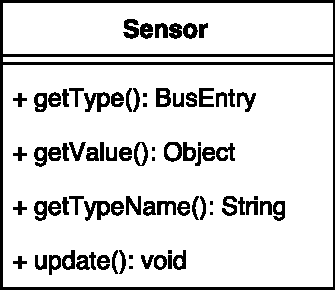
\includegraphics[width=0.4\textwidth]{SensorInterface.pdf}
	\caption{Sensor Architecture}
	\label{fig::si}
\end{figure}

\begin{itemize}
	\item \textbf{getType():} Returns a BusEntry. To pass the value to controller a databus is used where all values are kept in key-value pair manner. For data bus, keys are defined in BusEntry and for each sensor there should be a specific unique BusEntry. Main purpose of this method is to save the sensor value in the DataBus with getType() as a key and getValue() as value.  \\
	
	\item \textbf{getValue():} Returns the calculated value of the sensor. Before calling getValue() one should call update() method which calculates the value otherwise value would be null. The return type is kept as Object type because different kind of sensors produce different type of values. For example, camera sensor returns an Image object where velocity sensor returns Double object. The Object type of a sensor value can be get as String by calling getTypeName() method. \\
	
	\item \textbf{getTypeName():} It returns the object type of a sensor value. The type name is a String which contains full path of a Java Class like <package-name.Class-Name>. For example, for velocity sensor this method returns java.lang.Double on the other hand for camera sensor the type name will be java.awt.Image. \\
	
	\item \textbf{update():} It does not return anything but it contains the main calculation of the sensor. So, to produce sensor value on should call this method. \\
	
\end{itemize}
\subsection{Class Diagram}
\begin{figure}[H]
	\centering
	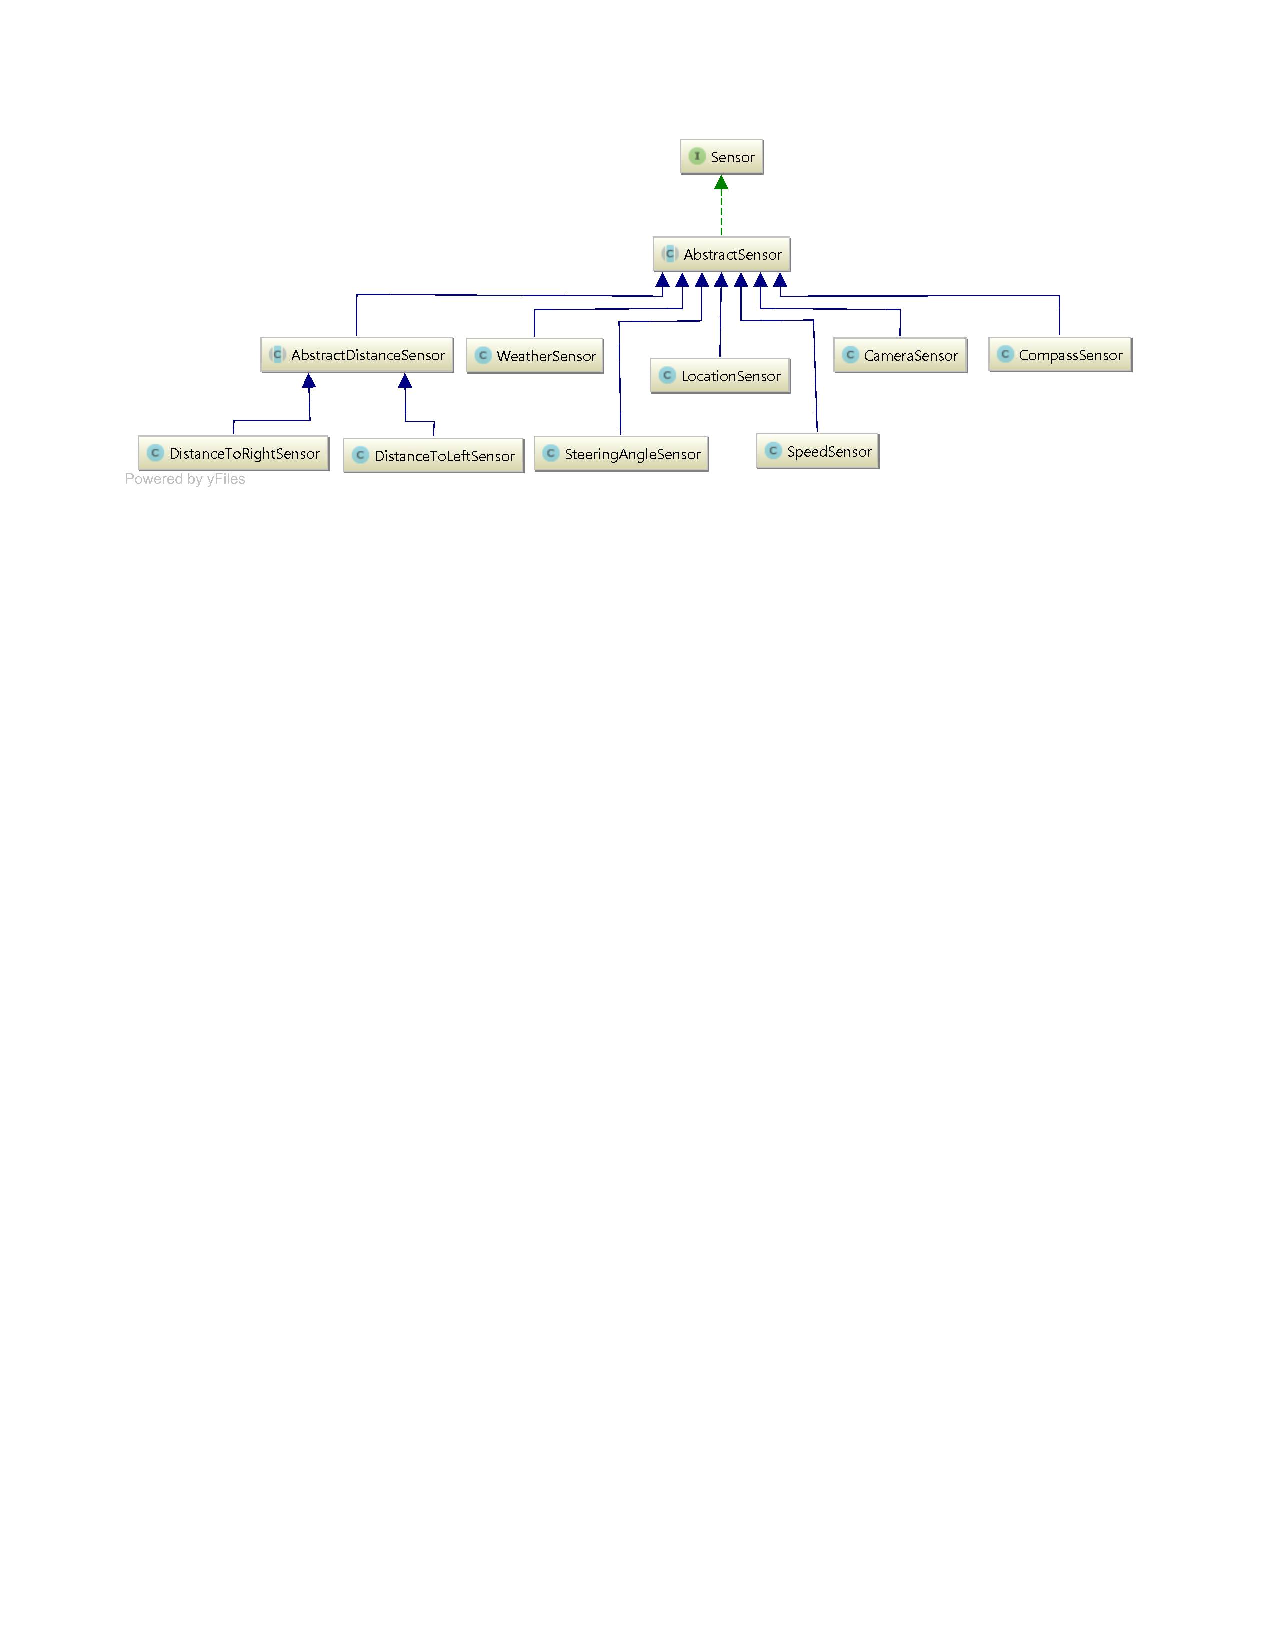
\includegraphics[scale=0.9]{diagram.pdf}
	\caption{Abstract Sensor}
	\label{fig::as}
\end{figure}
\subsection{Abstract Sensor}
It is an abstract class implementing the sensor interface. All sensors should extends this class. It has only one constructor. The constructor has one parameter which takes a Physicalvcehicle object as argument. This class also contains an abstract method called calculateValue(). The sensors who extends this update() class should have to implement calculateValue() method. This calculateValue() will contains the main calculation of the sensor. The update() method is implemented in this AbstractSensor class. In the update() method the calculateValue() is called. By this architecture one could put some checks in the update() method before calling calculateValue(). For example if someone creates a sensor Object with null Physicalvcehicle object, we can check before calling update if the  Physicalvcehicle object is null, and if it is null then calculateValue() method should not be called.

\section{Implemented Sensors}
All of the implemented sensors extends Abstract Sensor and each of them have one constructor which takes a Physicalvcehicle object.

    \subsection{SpeedSensor:}
    \begin{itemize}
        \item \textbf{Return value type:} java.lang.Double
        \item \textbf{Data Source:} Speed sensor extracts velocity value from physicalvehicle object which is a vector. After that, Norm\cite{Norm} function is applied in Velocity vector and converted to double value.
        \item \textbf{Noise Model:} The noise model for velocity assumed to be a Gaussian Distribution. With the standard deviation of 0.3, we generate a random value sampled from normal distribution and this value is chosen as calculated sensor value.
    \end{itemize}

    \subsection{SteeringAngleSensor:}
        \begin{itemize}
        \item \textbf{Return value type:} java.lang.Double
        \item \textbf{Data Source:} Extracts steering angle value from simulated vehicle object of physicalvehicle object. The value of steering angle we get from simulated vehicle is double.
        \item \textbf{Noise Model:} The noise model for SteeringAngle is same as velocity.
        \end{itemize}
    \subsection{LocationSensor:}
        \begin{itemize}
        \item \textbf{Return value type:} org.apache.commons.math3.linear.RealVector
        \item \textbf{Data Source:} Extracts position value from physicalvehicle object which is a vector.
        \item \textbf{Noise Model:} In real world, GPS sensor receives signal from satellite and based on the position of the satellite it calculates the vehicle position. So the accuracy of signal is highly depends on the weather and how satellite can see the GPS Module. For example, if one vehicle is in the under pass it is quite impossible to calculate the position of the vehicle. It is also true for bad weather. If it is snowing or storming, the value would be more inaccurate. For calculating the position of the vehicle we use Gaussian Distribution same as SpeedSensor but the standard deviation increase or decrease according to the weather condition.
        \end{itemize}
    \subsection{CameraSensor}
        \begin{itemize}
        \item \textbf{Return value type:} java.util.Optionalof(java.awt.Image)
        \item \textbf{Data Source:} Extracts Image from simulated vehicle object of physicalvehicle object. The image is in stereo mode[\ref{fig::stereo}]. First of all the stereo image is divided into two parts, one is the left image[\ref{fig::left_image}] an another is the right image. The default getValue() method will always returns the left image.
        \item \textbf{Noise Model:} The noise model of CameraSensor depends on motion of the vehicle. If vehicle is in very high speed, the captured image will have motion noise[\ref{fig:MotionBlur}]. Another noise could be perspective distortion of image[\ref{fig:Perspective}]. Currently those noise are not yet implemented because of performance. Those filters are applied in every pixel of the image and the processing becomes very slow. But the test cases are provided.
            \begin{figure}[H]
            	\centering
            	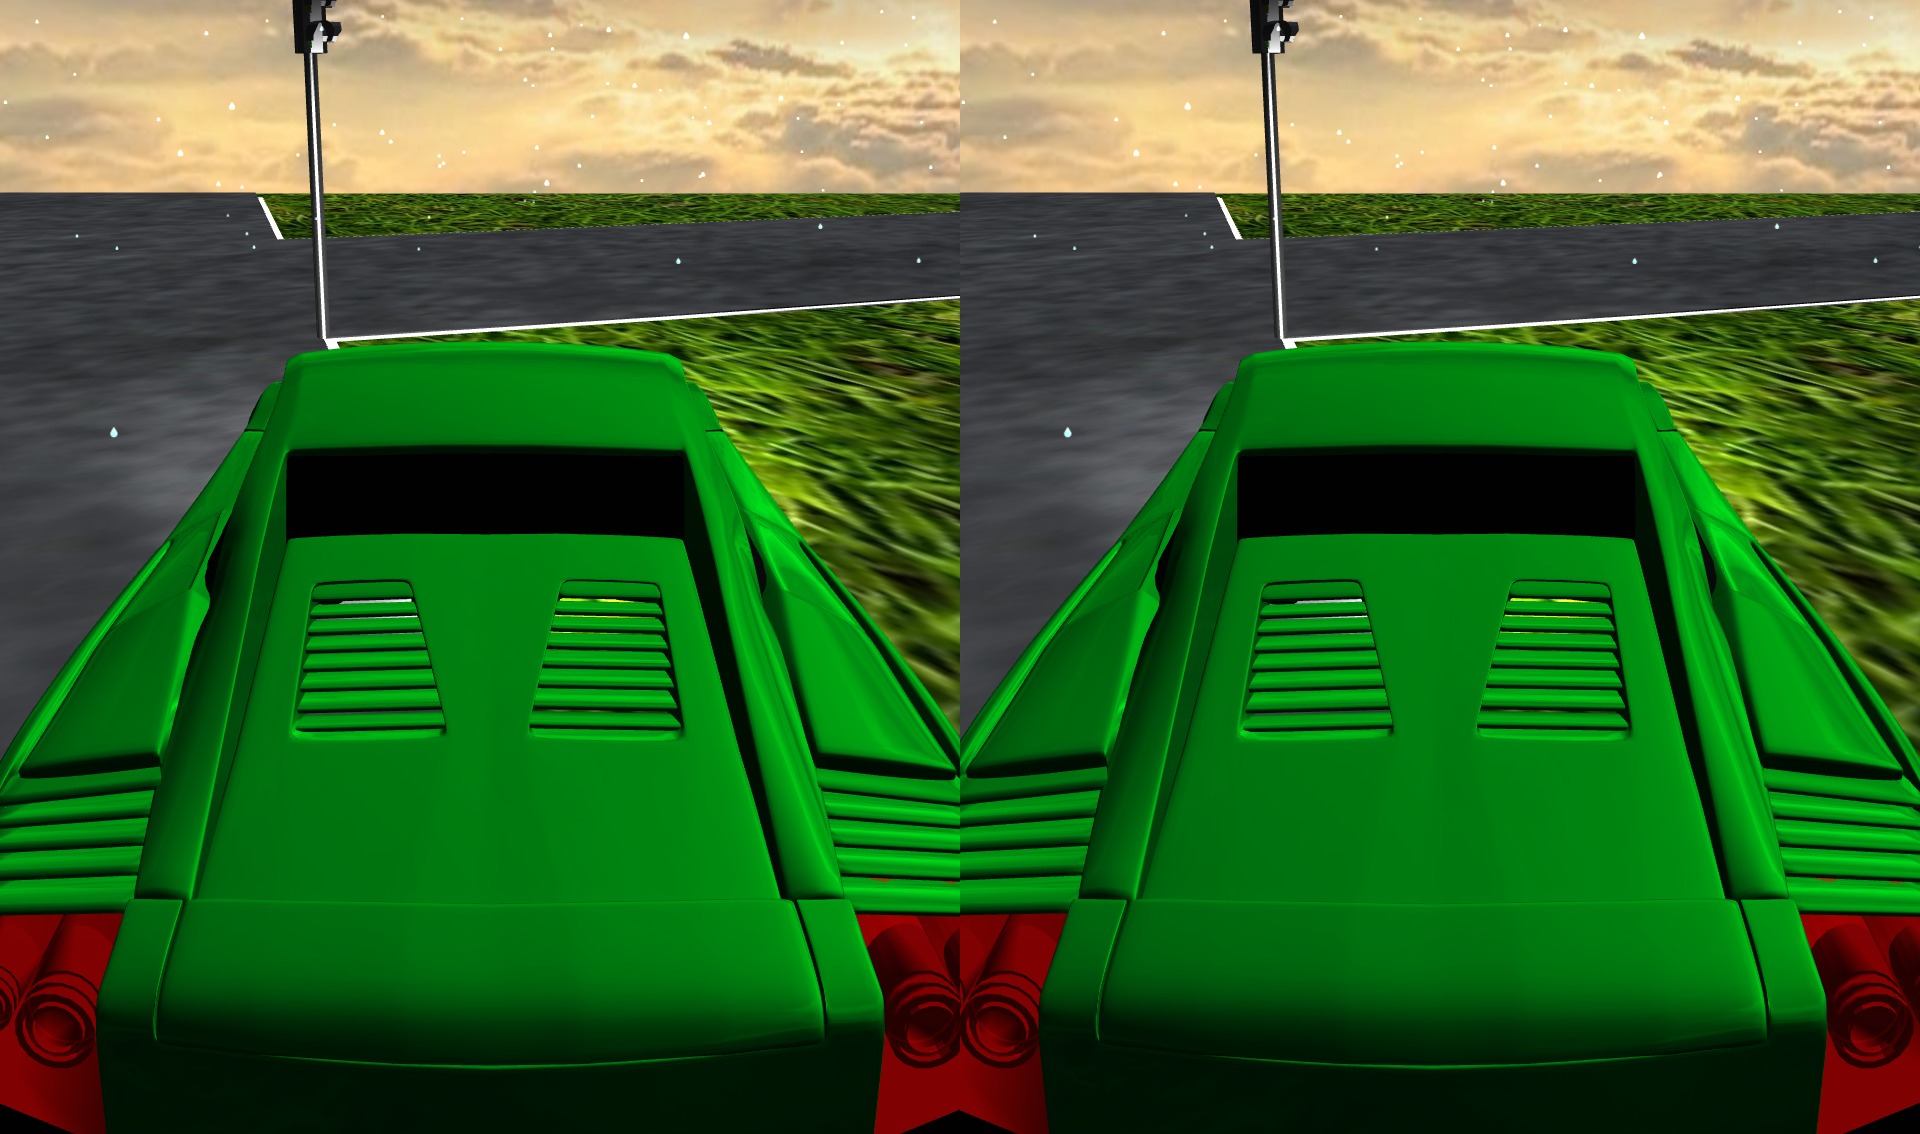
\includegraphics[width=0.8\textwidth]{Stereo_Image.jpg}
            	\caption{Extracted Stereo Image}
            	\label{fig::stereo}
            \end{figure}
            \begin{figure}[H]
            	\centering
            	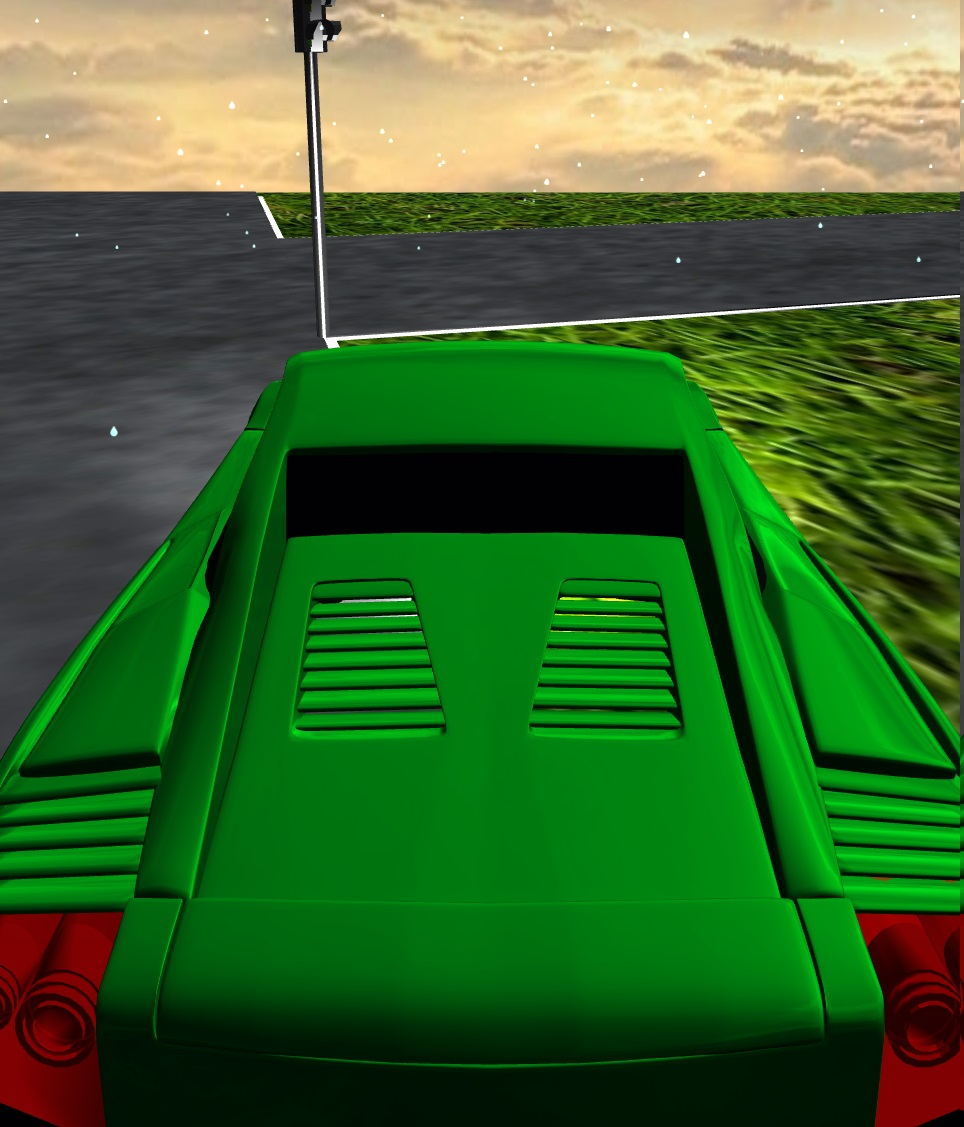
\includegraphics[width=0.4\textwidth]{left_Image.jpg}
            	\caption{Left image after Cropping}
            	\label{fig::left_image}
            \end{figure}
            \begin{figure}
            \centering
            \begin{minipage}{.5\textwidth}
              \centering
              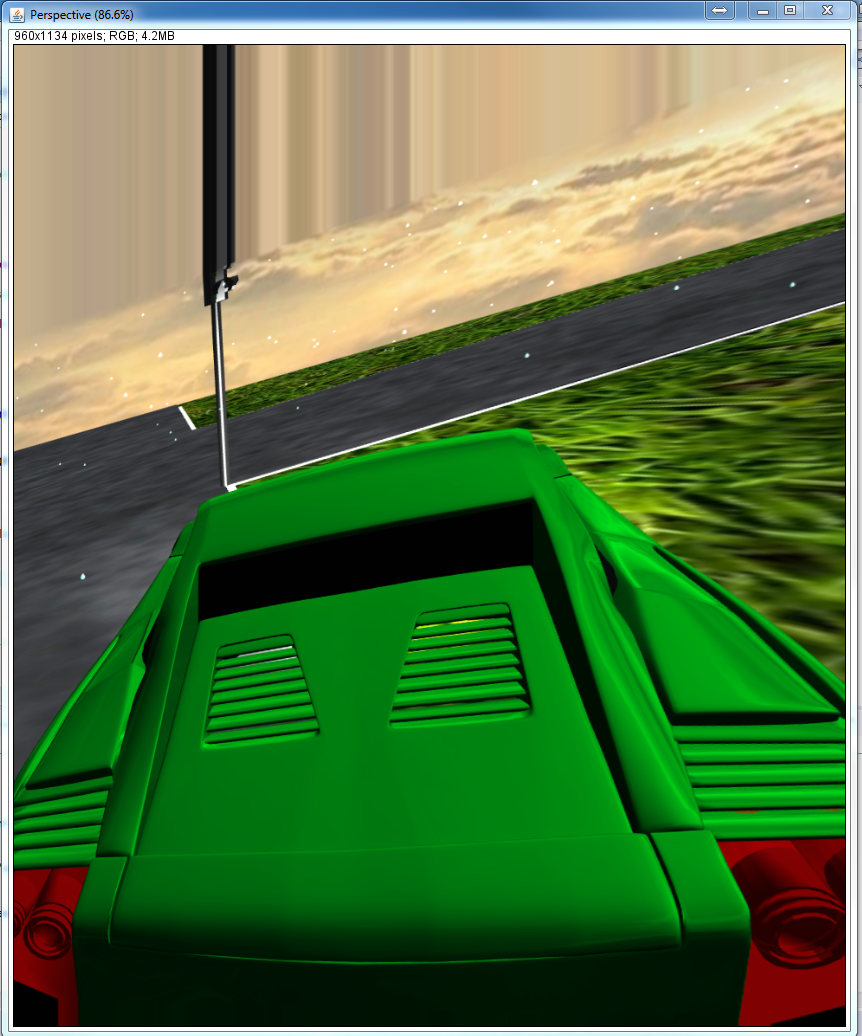
\includegraphics[width=.7\linewidth]{Perspective.png}
              \caption{Perspective Distortion}
              \label{fig:Perspective}
            \end{minipage}%
            \begin{minipage}{.5\textwidth}
              \centering
              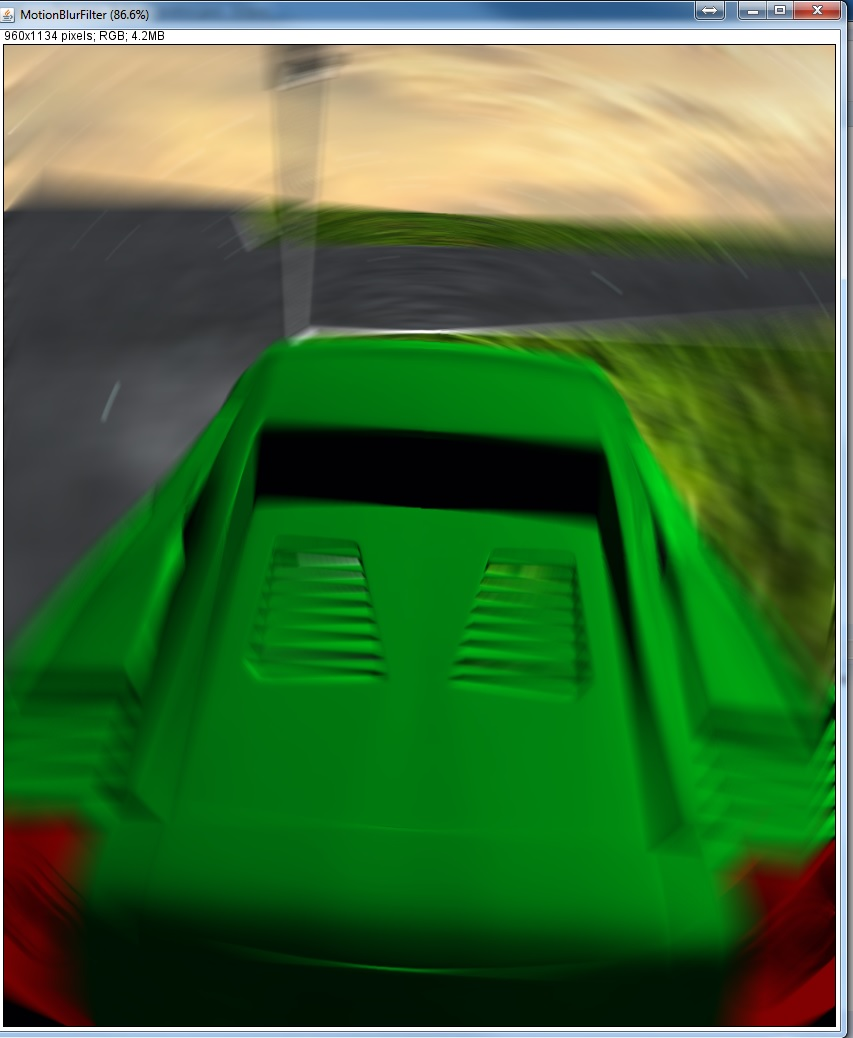
\includegraphics[width=.7\linewidth]{MotionBlur.jpg}
              \caption{Motion Blur Distortion}
              \label{fig:MotionBlur}
            \end{minipage}
            \end{figure}

            \end{itemize}

\newpage
\begin{thebibliography}{9}
\bibitem{Norm} 
Norm {https://books.google.com.au/books?id=hdkytqtBcyQC}
\end{thebibliography}

\end{document}
